%%-----------------Chapter 5---------------------------
\chapter{Verification and Validation} \labchap{verification_validation}
Now that we have an instrument designed, how can we determine if it meets requirements or not?
The system can be verified and then validated using a variety of techniques.
First, to verify that a requirement is present, the component or subsystem can be examined independently.
If it passes examination, we can update the traceability matrix to reflect that the requirement is now verified.
Once the feature is integrated with the entire system, then we can determine if it is validated or not.
Instead of examining the feature independently, it will be done so with the entire system to ensure that it functions properly.
These examinations can fall under four main types:

{
\renewcommand{\descriptionlabel}[1]{\hspace{\labelsep}\textbf{#1}}
\begin{description}
    \item[Inspection:] The nondestructive examination of a product or system using one or more of the five senses (visual, auditory, olfactory, tactile, taste). 
    It may also include simple physical manipulation and measurements.
    
    \item[Demonstration:] The manipulation of the product or system as it is intended to be used to verify that the results are as planned or expected.								
    
    \item[Test:] The verification of a product or system using a controlled and predefined series of inputs, data, or stimuli to ensure that the product or system will produce a very specific and predefined output as specified by the requirements.								
    
    \item[Analysis:] The verification of a product or system using models, calculations and testing equipment.
    Analysis allows someone to make predictive statements about the typical performance of a product or system based on the confirmed test results of a sample set or by combining the outcome of individual tests to conclude something new about the product or system.
    It is often used to predict the breaking point or failure of a product or system by using nondestructive tests to extrapolate the failure point.
\end{description}
}

For the following chapter, we shall examine each of Thetis' design capabilities from Tables \ref{tab:threshold_capabilities} through \ref{tab:stretch_capabilities} and verify their presence on the latest design.
Then, we shall do the same for the stakeholder requirements.

\section{Threshold Capabilities} \labsec{threshold_capabilities}

\newcommand{\yes}{\cellcolor[HTML]{63BE7B}Y}
\newcommand{\no}{\cellcolor[HTML]{F8696B}N}  %{0.9}

{\fontsize{8pt}{8pt}\selectfont
\begin{table}[ht!]
    \centering
	\renewcommand{\arraystretch}{1.5} % Set row height
	\begin{tabular}{| c | m{0.55\textwidth} | c | c | c |}
		\hline
		\multicolumn{5}{| c |}{\textbf{Threshold}} \\
		\hline
		\textbf{ID} & \multicolumn{1}{c|}{\textbf{Description}} & \textbf{Verified?} & \textbf{Validated?} & \textbf{Status} \\
		\hline
		101 & The system must be housed in an IP67-rated enclosure & \yes & \yes & D \\
		102 & The system enclosure must fit within the volume of 8" x 5" x 1.25" & \yes & \yes & D \\
		103 & The system software and firmware will be fully open-source & \yes & \yes & D \\
		104 & The system shall record inertial measurements at a minimum frequency of 64 Hz & \yes & \yes & D \\
		105 & The system shall be able to store data locally for up to 4 hours continuously & \yes & \no & TIP \\
		106 & The system shall be able to be operate for up to 4 hours continuously & \yes & \no & A \\
		107 & The system shall have simple human interface mechanism for status and logging & \yes & \yes & D \\
		108 & The system firmware shall be an open-architecture & \yes & \yes & A \\
		109 & The system will be fully documented & \no & \no & A \\
		110 & The system shall use version control software to track changes & \yes & \yes & D \\
		111 & The operator shall be able to offload data from the system & \yes & \yes & D \\
		112 & The system shall be capable of being assembled by hand using basic soldering tools & \yes & \yes & D \\
		\hline
	\end{tabular}
	\caption{Verification and validation of threshold capabilities}
	\labtab{vv_threshold_capabilities}
\end{table}
}

\paragraph*{101 - The system must be housed in an IP67-rated enclosure} This capability was initially verified by locating a suitable enclosure for Thetis and confirming with the manufacturer through the product data sheet that the system was properly rated.
Then, it was validated by placing the enclosure onto a Remotely Operated Vehicle (ROV) and descending down to 20-feet of depth while the ROV performed a mission.
Paper towels were placed within the enclosure so that if any water breached the seals, it would be immediately apparent.
This represented a worst-case scenario and the enclosure held its seal meaning that it exceeded the capability requirement.

\begin{figure}[h!]
    \caption[ROV Setup]{Thetis (bottom) attached to a Blue ROV2 frame for enclosure testing.}
    \labfig{thetis_rov}
    \centering
    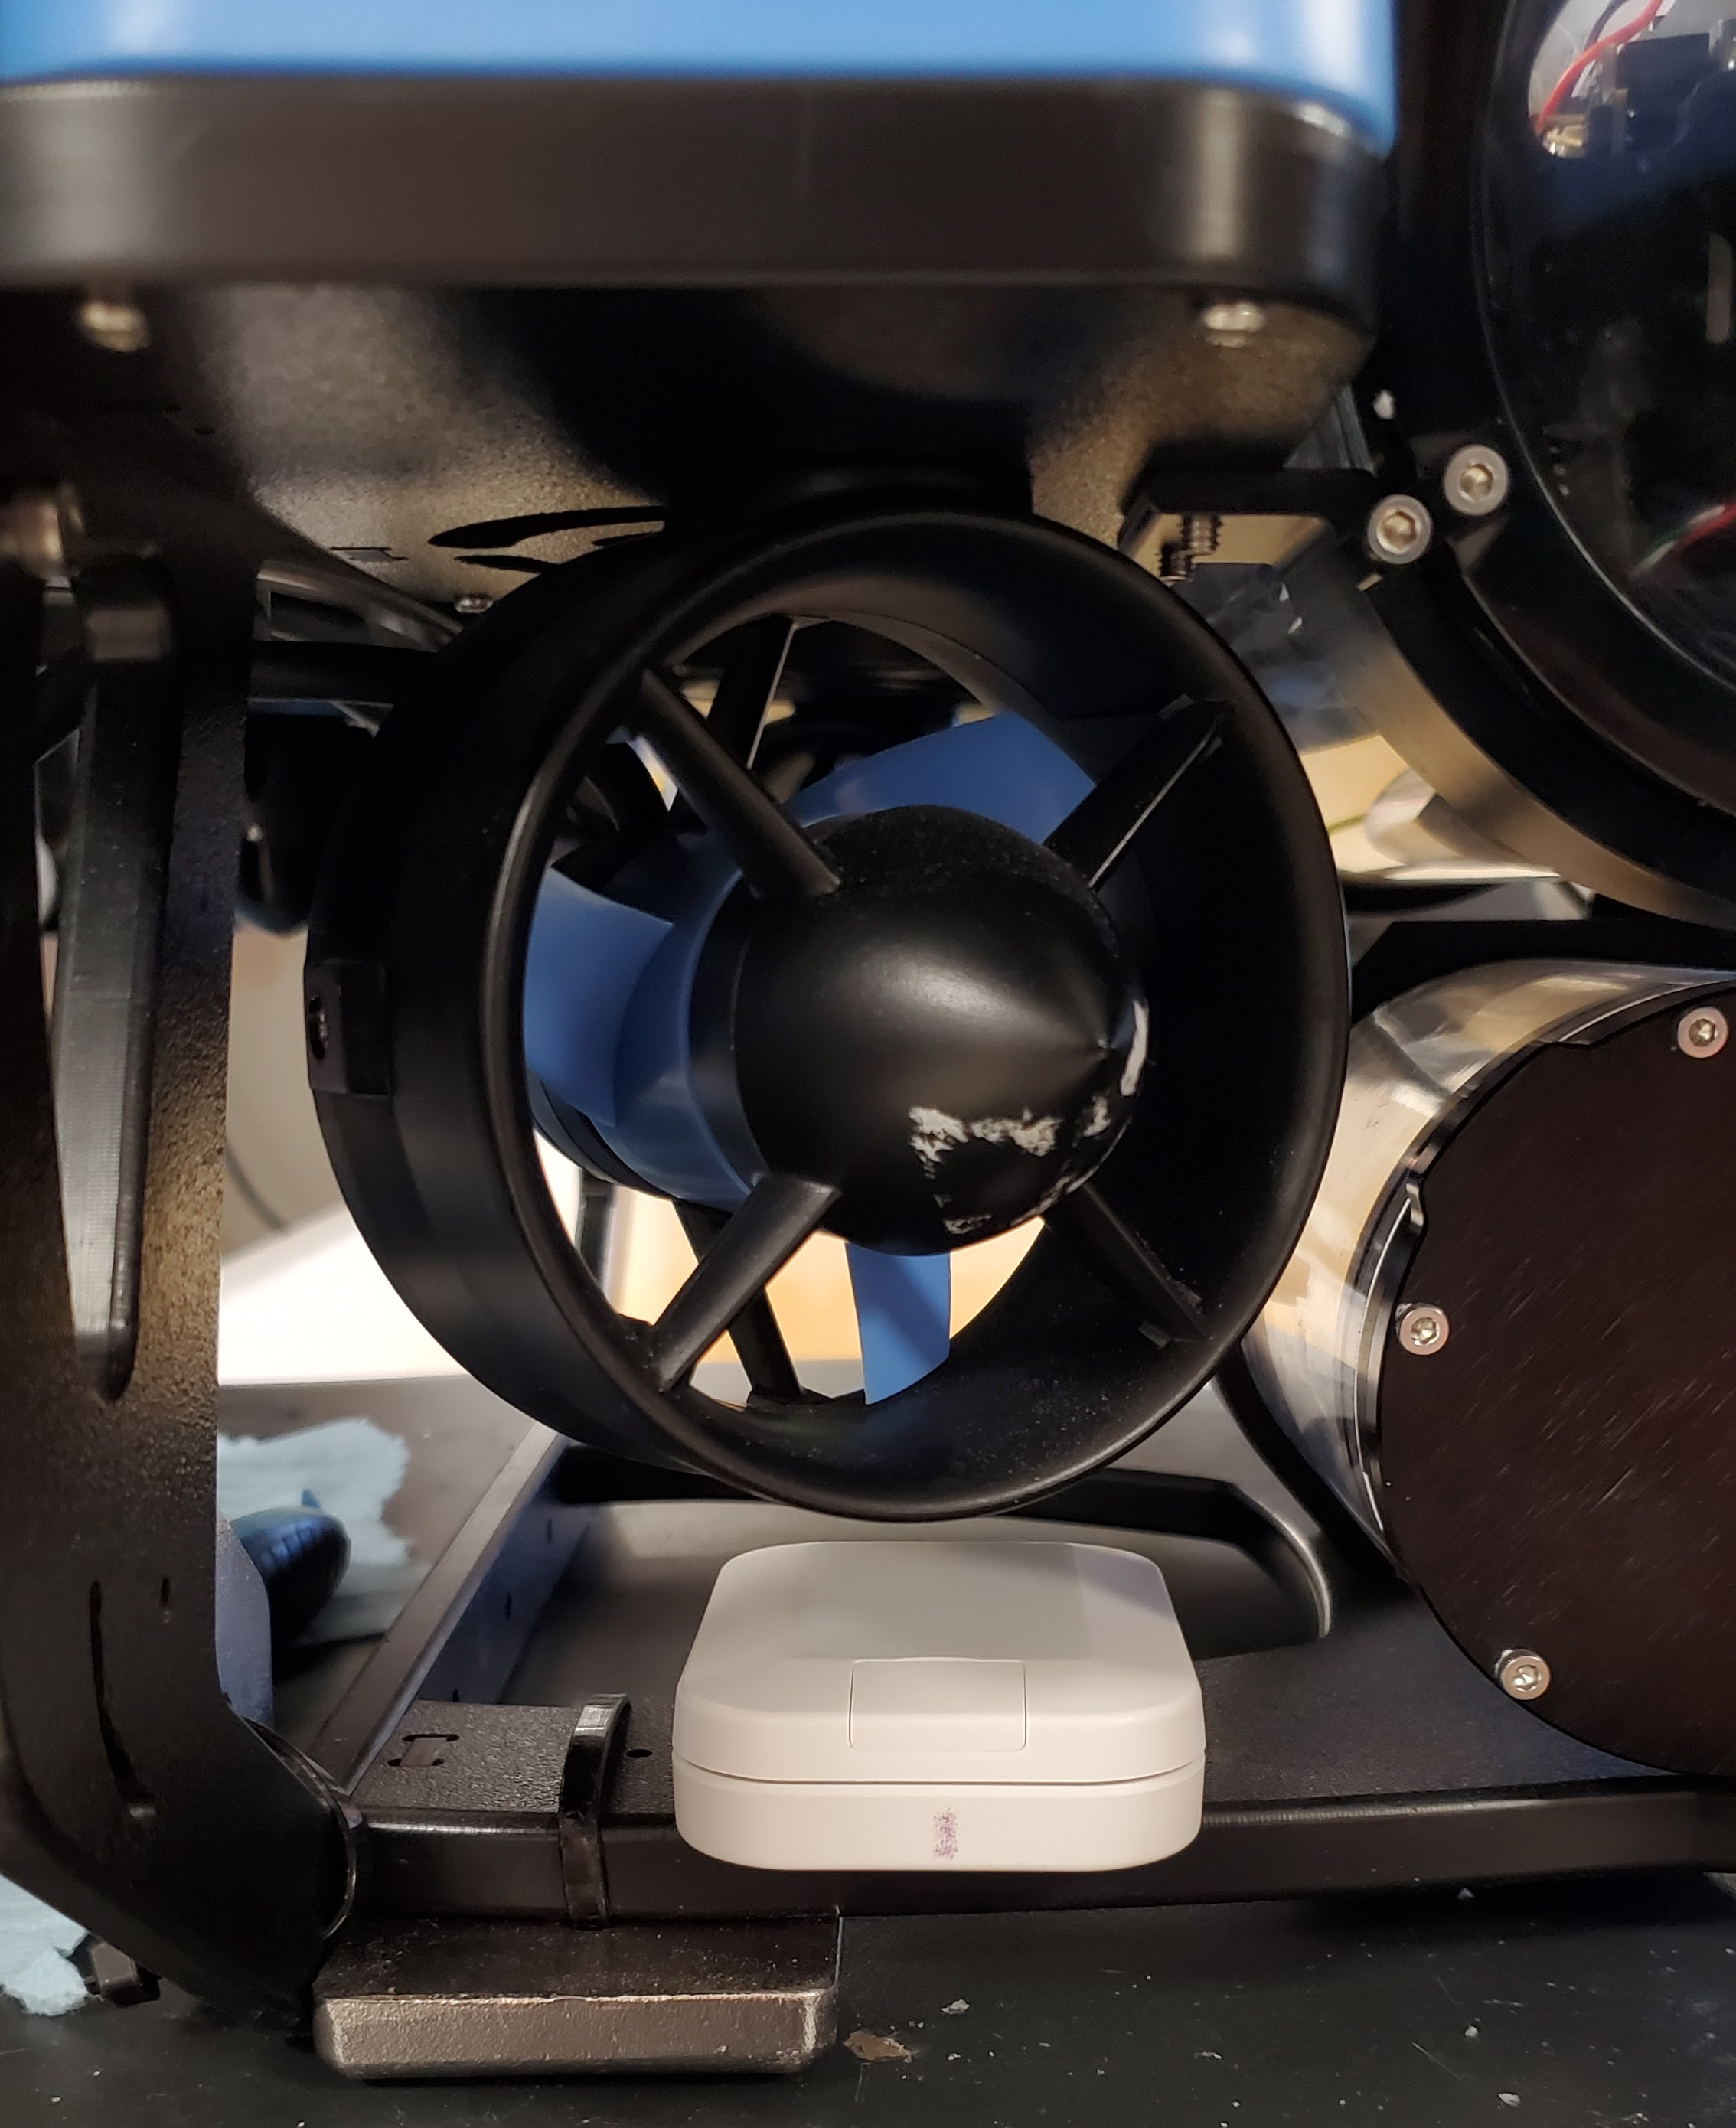
\includegraphics[height=2.5in]{verify_validate/thetis_rov.jpg}
\end{figure}

To represent a more realistic use case, Thetis was placed into a cutout on a surfboard and deployed into the ocean to catch some waves.
Out nine separate deployments, the case seal failed three different times:

\begin{enumerate}
    \item A screw was not present in one corner, thereby not clamping that section of the sealing material, 
    \item a screw was over-torqued and caused the area around the screw to crack, bypassing the seal, and 
    \item the same case as before was used accidentally.
\end{enumerate}

All three failures were due to operator error proving that careful procedures need to be implemented for actual deployments.
However, when the case was properly sealed by operators, the seals held and the electronics within were not damaged, even when completely submerged and subjected to dynamic forces as the surfboard rolled and slammed into waves.

\begin{figure}[h!]
    \caption[Surfboard Setup]{Thetis (right) and the x-IMU3 (left) secured in a cutout on a modified surfboard during a deployment.}
    \labfig{thetis_surfboard}
    \centering
    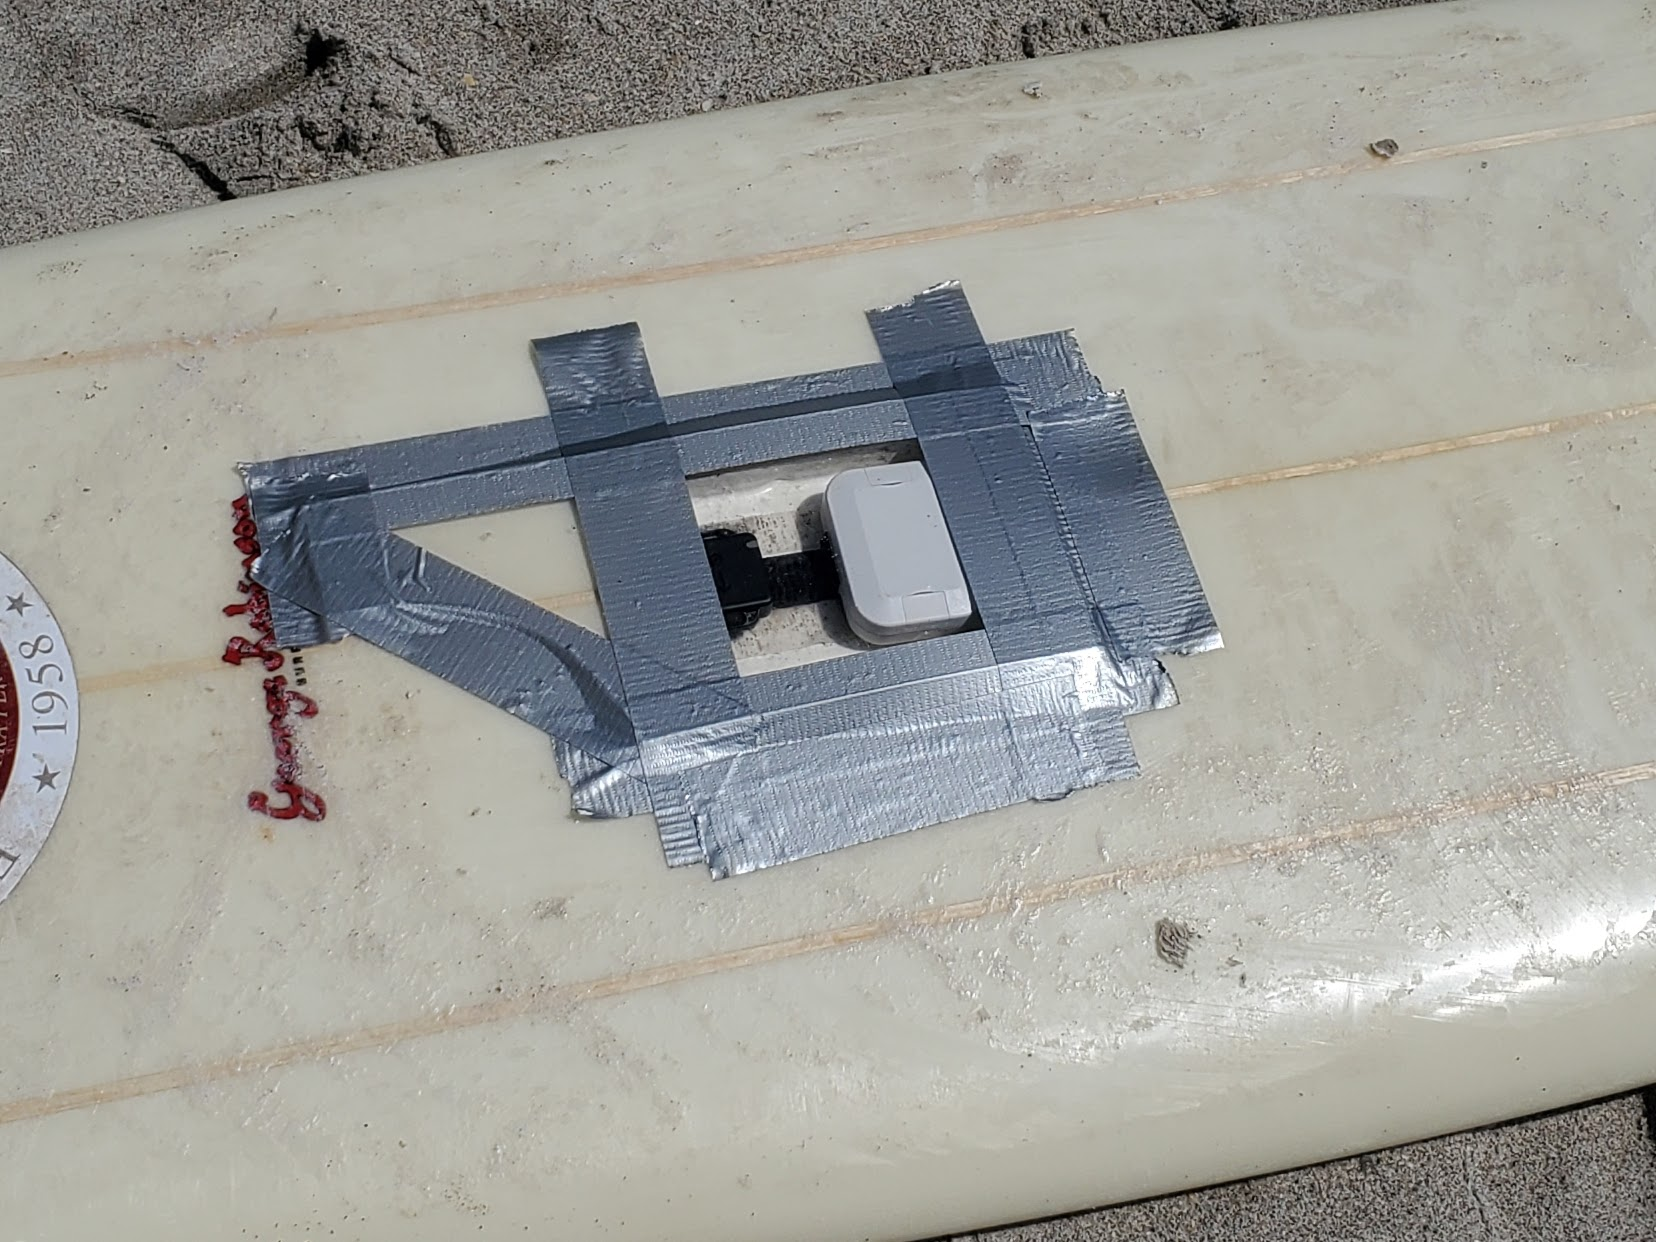
\includegraphics[height=2.5in]{verify_validate/thetis_surfboard.jpg}
\end{figure}

\paragraph*{102 - The system enclosure must fit within a volume of 8" x 5" x 1.25"} Like Capability 101, this was initially verified by inspection during the search for this enclosure and confirming the enclosure dimensions with the manufacturer.
Then, it was validated by placing it securely into the cutouts in the surfboard made for the iPhone 6S - the device Thetis is intended to replace, as shown in Figure \ref{fig:thetis_surfboard}.

\paragraph*{103 - The system software and firmware will be fully open-source} This capability is both verified and validated by inspection as the code is readily accessible on GitHub.
The firmware is broken into several sub repositories: \href{https://github.com/Legohead259/Thetis-Firmware}{Thetis-Firmware}, \href{https://github.com/Legohead259/ThetisLib}{ThetisLib}, \href{https://github.com/Legohead259/xioAPI-Arduino}{xioAPI-Arduino}, \href{https://github.com/Legohead259/Timer-Events-Arduino}{Timer-Events-Arduino}, and \href{https://github.com/Legohead259/Fusion-Arduino}{Fusion-Arduino} all of which are under the MIT license and available.
Thetis has several tangential software packages that are also open source such as the \href{https://github.com/Legohead259/Thetis-Scripts}{scripts repository} used for data processing and analysis, the \href{https://github.com/xioTechnologies/x-IMU3-Software}{x-IMU3 GUI} used to visualize data and log from a host computer, and the \href{https://github.com/Legohead259/Thetis-Calibration}{code for the calibration machine}.

\paragraph*{104 - The system shall record inertial measurements at a minimum frequency of 64 Hz} This capability requires a demonstration in order to be verified and validated.
We can initially inspect the firmware to ensure that the inertial measurements are taken every 15.6 milliseconds, but it is not guaranteed that the system can consistently take measurements at that speed.
Therefore, the best way to demonstrate this capability was during the calibration procedure detailed in Section \ref{sec:calibration_methodologies}.
Thetis was set to record at 64 Hz and when the data was offloaded, it was confirmed to be taken at the appropriate interval.
Therefore, this capability has been verified and validated within the system.

\paragraph*{105 - The system shall be able to data locally for up to 4 hours continuously} We can analyze the size of logging messages and SD card to determine if this capability is verified.
In the latest version of the firmware, five messages are published to the data storage device: position, inertial, magnetic, quaternion, and euler angle.
Combined, these messages take 198 bytes of space and occur, on average, 64 times per second for 12,672 bytes per second.
There are 14,400 seconds in 4 hours, so multiplying these values together, we get 182.5 megabytes of storage required for 4 hours of use.
The microSD cards used throughout testing are at least 4 gigabytes which gives an estimated 88 hours of continuous logging.
This requirement was validated by running Thetis for four hours continuously and verifying that the log file was successfully created and maintained for that period.

\begin{equation} \labeq{storage_time}
    t_{\text{samples}} = \frac{N_{\text{storage}} [\text{Bytes}]}{198 [\text{Bytes}] \times 64 [\text{s}^{-1}] \times 3600 \left[\frac{\text{s}}{\text{h}}\right]} = \frac{4 [\text{GB}]}{198 [\text{Bytes}] \times 64 [\text{s}^{-1}] \times 3600 \left[\frac{\text{s}}{\text{h}}\right]} = ~88 [\text{h}]
\end{equation}

\paragraph*{106 - The system shall be able to operate for up to 4 hours continuously} For this capability, we can verify it by analysis like the previous one.
We need to start with a couple of assumptions:

\begin{enumerate}
    \item Battery capacity is 420 mAh with 3.7V nominal voltage,
    \item Current consumption without WiFi enabled is ~50 mA, and
    \item Current consumption with WiFi enabled is ~120 mA while transmitting
\end{enumerate}

The latter two assumptions are based on a zeroth-order estimate by summing together the estimated current consumption of the various components as listed in their data sheets.
We can then make a zeroth-order estimate using Equation \ref{eq:battery_life}.
This yields an estimated continuous battery life of 9.4 hours without WiFi and 3.9 hours with WiFi.
An important note about the WiFi estimate is the assumption that it is constantly transmitting.
In reality, this may not be accurate so the battery life may be longer.
If it is below the four-hour threshold, then certain mitigations can be implemented like a burst-mode transmission of data every couple of second or minutes.

\begin{equation} \labeq{battery_life}
    t_{\text{battery}} = \frac{3.7 [\text{v}] \times 420 [\text{mAh}]}{3.3 [\text{V}] \times I_{\text{mode}} [\text{mA}]}
\end{equation}

This capability was validated by running Thetis for four hours continuously from full battery power and ensuring that the battery voltage at the end of the test was within the safe operating limits.
Specific power consumption tests were not performed due to the technical complexity of precisely measuring current draw.

\paragraph*{107 - The system shall have a simple human interface mechanism for status and logging} This is another capability that is straight forward to verify and validate using inspection techniques.
First, to enable logging, an operator only needs to hold the ``log'' button for a half second and the same to stop logging.
To convey status, the RGB LED on-board changes color and pattern.
By referencing the current RGB LED color and pattern with the diagnostic LED table, then the operator can know what the system is doing.
These features were used extensively throughout testing with great success.

\paragraph*{108 - The firmware shall be open architecture} This capability is challenging to fully define and implement, hence its relatively low priority in the threshold category.
To verify this capability has been met, we should consider the difficulty of adding a new feature or component to the firmware.
The firmware uses an object-oriented approach with a star topology.
This means that a new feature can be added by putting it into the appropriate class and tying it to other classes/functions through the main \lstinline[style=customInline]|Thetis| object.
Similarly, we can add a new component by creating a new class in the library and then implementing it in the main class.

Validating this capability will require more research out the scope of this thesis to ensure a proper software architecture is implemented and followed.

\paragraph*{109 - The system will be fully documented} This is another capability that is easy to validate and verify through testing.
Multiple groups of students and stakeholders will be asked to perform simple tasks using Thetis such as replacing a component, assembling the board, adding a firmware feature, or performing calibration.
If the participants are able to perform the task using the available documentation, then this capability has been verified and validated.
Otherwise, the documentation needs to created or modified accordingly.

\paragraph*{110 - The system shall use version control software to track changes} As discussed in Section \ref{ssec:version_control}, GitHub is a centralized VCS solution that enables version history and tracking.
Since all of the software and firmware for Thetis is on GitHub, this capability has been thoroughly verified and validated.
Similarly, all of the hardware was designed in Fusion 360 which implements its own VCS solution and then backed up to GitHub.

\paragraph*{111 - The operator shall be able to offload data from the system} Since the operator needs to be able to pull data off the system after an experiment, this capability is easily verified and validated via demonstration.
During the calibration procedure, data was routinely written to the onboard microSD card and then the operator could pull the card out, load it into a host computer, then transfer the data into an analysis script.
Additionally, data was able to be recorded in real-time through the x-IMU3 GUI application on a host computer through a USB connection to Thetis.
Both of these methods and verified that the capability was implemented and the fact that it could be reliably used throughout multiple tests validated it.

\paragraph*{112 - The system shall be capable of being assembled using basic soldering tools} This capability was clearly demonstrated in Section \ref{ssec:assembly_techniques} where the board is shown to be assembled using solder paste, tweezers, a soldering iron, and hot air.
We can also verify this capability by inspecting the various component used throughout the design.
The smallest component is an `0603' which is 60 thousandths of an inch long by 30 thousandths wide.
While certainly small, they can be manipulated by a steady hand and placed on the board with reasonable accuracy.
For these reasons, this capability has been verified and validated.

\section{Reach Capabilities}

{\fontsize{8pt}{8pt}\selectfont
\begin{table}[ht!]
    \centering
	\renewcommand{\arraystretch}{1.5} % Set row height
	\begin{tabular}{| c | m{0.55\textwidth} | c | c | c |}
		\hline
		\multicolumn{5}{| c |}{\textbf{Reach}} \\
		\hline
		\textbf{ID} & \multicolumn{1}{c|}{\textbf{Description}} & \textbf{Verified?} & \textbf{Validated?} & \textbf{Status} \\
		\hline
		201 & The system shall use a GPS with a minimum 1 Hz update rate for position tracking & \yes & \no & TIP \\
		202 & The system will have a simple logging and status interface accessible via web terminal & \no & \no & A \\
		203 & The system shall be able to monitor and report battery state of charge & \yes & \no & A \\
		204 & The system will have configurable settings that can be changed by the operator & \yes & \yes & D \\
		205 & The system can operate in a Wi-Fi access point or client mode	& \yes & \no & A \\
		206 & The sensor measurements shall incorporate a calibration model & \yes & \no & TIP \\
		\hline
	\end{tabular}
	\caption{Verification and validation of reach capabilities}
	\labtab{vv_reach_capabilities}
\end{table}
}

\paragraph*{201 - The system shall use a GPS with a minimum 1 Hz update rate for position tracking} This capability can be verified by inspecting the GPS used on Thetis.
The GPS receiver uses the MTK3339 chipset\footnote{\url{https://www.adafruit.com/product/746}} which is capable of update messages every 1 to 10 Hz, according to its manufacturer data sheet. 
This feature was validated by placing Thetis at a monument \footnote{\url{https://ngs.noaa.gov/cgi-bin/ds_mark.prl?PidBox=AK4011}} with a known GPS coordinate for one hour.
Readings were taken at 1 Hz and recorded to the data log file.
Figure \ref{fig:gps_error} shows the distribution of measurement errors over the test in Northings and Eastings and the calibration script and data can be found in \cite{Thetis-Scripts}.

The measurement plot shows that 95\% of the GPS measurements fall within 5-meters of the known GPS position.
This is slightly worse performance than typically expected (about 3-meters \cite{Hofmann:2001}) but can be attributed to the small chip antenna on top of the module and the unoptimized PCB layout.
On Revision F5, the GPS module has a broken ground plane beneath it.
This results in RF noise and attenuation within the module that will decrease its accuracy.
This issue is addressed in Revision F6 (\ref{ssec:future_hardware}).
The drifting readings to the south east are aslo interesting and should be further investigated.

\begin{figure}[h!]
    \caption{GPS measurement deviations as measured from Thetis Revision F5 in middle of the day, clear conditions.
	Expected error should be less than 3-meters}
    \labfig{gps_error}
    \centering
    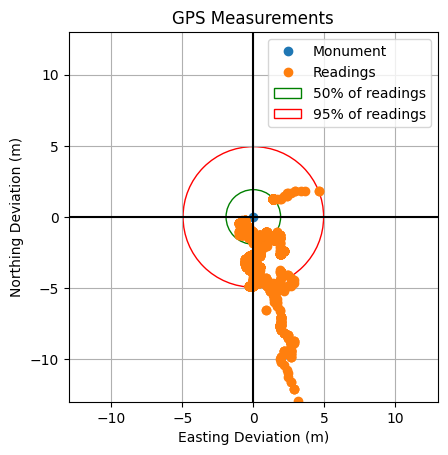
\includegraphics[height=2.5in]{verify_validate/gps_test_errors.png}
\end{figure}

\paragraph*{202 - The system will have a simple human interface accessible via web browser} In earlier versions of the firmware, there was a basic webpage that allowed operators to start/stop logging and check the device status.
However, in the latest firmware version, this capability was removed to simplify testing.
The hardware is still capable of providing this interface but it remains to be implemented.
For more information, see Section \ref{ssec:future_wireless}.

\paragraph*{203 - The system shall be able to monitor and report battery state of charge} This capability has been verified through inspection by integrating the MAX17048 \footnote{\url{https://www.digikey.com/en/products/detail/analog-devices-inc-maxim-integrated/MAX17048G-T10/3758921}} onto the board design.
This chip calculates state of charge and reports it to the microcontroller.
Then the battery state is reported as a battery message through the device API.
However, this capability has not been validated as the battery monitor chip has not been calibrated for the selected batteries nor analyzed for its accuracy.
Further testing is required as detailed in Section \ref{ssec:future_settings} and \ref{ssec:future_vv_power}.

\paragraph*{204 - The system will have configurable settings that can be changed by the operator} This capability was another one that was verified and validated throughout the calibration process by testing.
The firmware implements and extends the xioAPI which provides an extensive list of settings that can be changed via JSON commands \cite{ThetisUserManual}.
The calibration process required tweaks to some settings which were routinely done through the USB connection to a host computer.
Additionally, during development of this feature, every setting was tested and validated to work.

\paragraph*{205 - The system can operate in a Wi-Fi access point or client mode} This capability can be verified by inspecting the manufacturer data sheet for the microcontroller used on Thetis.
The ESP32 series of chips used on the board are Wi-Fi enabled microcontrollers that can broadcast their own networks (access point mode) or connect to a local one (client mode).
On Thetis, switching between these modes and Wi-Fi disabled is done through configuration commands.
Performance of the Wi-Fi connection and other features have not been validated in the latest firmware and should be integrated following the discussion in Section \ref{ssec:future_wireless} and \ref{ssec:future_vv_wireless}.

\paragraph*{206 - The sensor measurements shall incorporate a calibration model} The capability is implemented by using the Madgwick sensor fusion algorithm described in Chapter \ref{chap:background} and the \lstinline[style=customInline]|Fusion| library made for that algorithm.
The \lstinline[style=customInline]|Fusion| library incorporates the calibration model described in Equations \ref{eq:inertial_model} and \ref{eq:magnetic_model} by default and the specific calibration parameters are loaded as configuration settings.
Due to the failure of the calibration process, this capability was not validated.

\section{Stretch Capabilities}

{\fontsize{8pt}{8pt}\selectfont
\begin{table}[ht!]
    \centering
	\renewcommand{\arraystretch}{1.5} % Set row height
	\begin{tabular}{| c | m{0.55\textwidth} | c | c | c |}
		\hline
		\multicolumn{5}{| c |}{\textbf{Stretch}} \\
		\hline
		\textbf{ID} & \multicolumn{1}{c|}{\textbf{Description}} & \textbf{Verified?} & \textbf{Validated?} & \textbf{Status} \\
		\hline
		301 & The system file storage shall be accessible via web or USB interface	& \no & \no & A \\
		302 & The system shall have a backup storage option in case primary storage fails & \no & \no & R \\
		303 & The system will use a microcontroller capable of machine learning using TinyML & \no & \no & UR \\
		304 & The system shall be able to log in a burst mode for up to 24 hours & \no & \no & UR \\
		\hline
	\end{tabular}
	\caption{Verification and validation of stretch capabilities}
	\labtab{vv_stretch_capabilities}
\end{table}
}

\paragraph*{301 - The system file storage shall be accessible via web or USB interface} From previous experiments with the ESP32-S2 and -S3 microcontrollers, it is possible to host a File Transfer Protocol (FTP) server \footnote{\url{https://www.mischianti.org/2020/02/08/ftp-server-on-esp8266-and-esp32}} or have the device appear as a USB flash drive \footnote{\url{https://github.com/Legohead259/ThetisLib/blob/ba94c8f8eba002fef2d88b5f21aa544ef2b5b2b1/Examples/usbmsc/test.ino}} when connected to a host computer.
However, in the latest firmware version, these features are not implemented so this capability is feasible, but not verified or validated in the current system.

\paragraph*{302 - The system shall have a backup storage option in case primary storage fails} This capability was initially envisioned as a mitigation for any microSD card failure mode.
Especially in cases where the microSD card could become physically damaged during a test, the secondary option would still allow some data to be recovered.
However, as explained in \ref{sec:prototype_problems}, this capability introduced system-breaking errors and the anticipated failure mode was never encountered throughout initial testing.
Therefore, this capability was rejected in favor of a simplified and more reliable software and hardware design.

\paragraph*{303 - The system will use a microcontroller capable of machine learning using TinyML} This capability was added to address some of the future efforts proposed in the next chapter.
An experiment was run \footnote{\url{https://github.com/Legohead259/Project-Thetis-TinyML-Example}} that proved the feasibility, but due to the technical effort and time constraints, this capability was not seriously considered for implementation.

\paragraph*{304 - The system shall be able to log in a burst mode for up to 24 hours} This is another capability that was envision for a future use, but never seriously considered for implementation.
The idea with this is to extend the battery life to capture inertial signals over a longer time span such as required for the WEAVE experiment proposed in Section \ref{chap:weave}.
However, this capability could be better implemented by a new hardware revision that could accept external battery power, instead of relying on its smaller internal battery.
Theoretically, this is possible to integrate using the component's sleep functionalities and other techniques.

\section{Stakeholder Requirements}

{\fontsize{8pt}{8pt}\selectfont
\begin{table}
	\centering
	\renewcommand{\arraystretch}{1.75}
	\begin{tabular}{|c | m{0.5\textwidth} | c | c | c |}
		\hline
		\textbf{ID} & \multicolumn{1}{c |}{\textbf{Description}} & \textbf{Verified?} & \textbf{Validated?} & \textbf{Status} \\
		\hline
		SR 01 & The system shall be able to record acceleration, rotation rate, orientation, and position & \yes & \yes & TIP \\
		SR 02 & The system shall be able to fit into a small IP67-rated, or better, enclosure & \yes & \yes & D \\
		SR 03 & The system shall be able to be powered by battery for more than 4 hours continuously & \yes & \yes & D \\
		SR 04 & The system shall be cheaper than \$200 per unit & \yes & \no & A \\
		SR 05 & The system shall use components that are readily available COTS & \yes & \yes & D \\
		SR 06 & The system designs shall be open source for modification by students & \yes & \yes & D \\
		SR 07 & The system shall allow users to change settings via interface and/or configuration file & \yes & \yes & D \\
		SR 08 & The system shall communicate extra-device using WiFi and USB & \yes & \yes & A \\
		SR 09 & They system shall have enough on-board storage for 4 hours of continuously logging at 64 Hz & \yes & \yes & D \\
		\hline
	\end{tabular}
	\caption{Verification and validation of stakeholder requirements}
	\labtab{vv_stakeholder_reqs}
\end{table}
}

\paragraph*{SR 01 - The system shall be able to record acceleration, rotation rate, orientation, and position} The requirement was verified and validated throughout the calibration procedure described in the previous chapter.
Thetis recorded and output the inertial measurements (rotation rate and acceleration), magnetometer readings, position measurements from the GPS, and orientation as both a quaternion and euler angles.
This was recorded through the on-board microSD card logger and through the x-IMU3 GUI application running on a host computer and connected via USB.

\paragraph*{SR 02 - The system shall be able to fit into a small IP67-rated, or better, enclosure} As explained with Capabilities 101 and 102 in Section \ref{sec:threshold_capabilities}, this requirement was verified and validated by testing the enclosure at depth on an ROV and in a more realistic deployment.
The enclosure held a water-tight seal when properly engaged and undamaged.

\paragraph*{SR 03 - The system shall be able to be powered by battery for more than 4 hours continuously} This requirement was verified using the analysis discussed in Section \ref{sec:threshold_capabilities} with Capability 106. 
It was further validated by running the system for more than 4 hours and checking that the end battery voltage was at an acceptable level.

\paragraph*{SR 04 - The system shall be cheaper than \$200 per unit} This requirement was verified by inspecting the Bill of Materials for Thetis and checking that the summation was less than \$200.
This requirement is difficult to validate however, because additional hardware revisions may be necessary to improve performance or add additional features.
This estimate also does not include the development time or overall expense, which would definitely increase the unit price.

\paragraph*{SR 05 - The system shall use components that are readily available COTS} This requirement was verified and validated by sourcing components from online distributors like DigiKey.
All of the components used on Thetis can be purchased online and then assembled on the custom PCB. 
This requirement was tricky to implement during the chip shortage of 2020, but now that more components are more readily available, further hardware revisions should not have any problems continuing to use COTS parts.

\paragraph*{SR 06 - The system shall be open source for modification by students} This requirement is verified by the extensive use of GitHub repositories that are public-facing and accessible by anyone with an internet connection.
Students can access the repositories, download the source code and files, make modifications as needed.
To validate the requirement, multiple groups of students and stakeholders were gathered to attempt various tasks such as repair a chip, calibrate the board, add a new software feature, etc.
As they were performing these tasks, they were given documentation and in turn provided feedback on the quality of the documentation and any clarifications they needed.

\paragraph*{SR 07 - The system shall allow users to change settings via interface and/or configuration files} The requirement was verified by implementing and extending the xioAPI in the Thetis firmware.
This API provides a suite of settings to control how the board performs and its capabilities.
The configurations can be changed via a web or USB interface to a host computer or by uploading a custom configuration file to the onboard flash storage.
To validate the requirement, each setting was thoroughly tested to ensure it could be changed and the interface was used during the calibration process to tweak a couple of settings.

\paragraph*{SR 08 - The system shall communicate extra-device using Wi-Fi and USB} Since Thetis uses a microcontroller that is capable of USB host and Wi-Fi, this requirement is easily verified by inspecting the manufacturer data sheet.
However, the requirement remains unvalidated because the performance when using the wireless interface is severely limited.
More testing is required as detailed in Section \ref{ssec:future_wireless} and \ref{ssec:future_vv_wireless}

\paragraph*{SR 09 - The system shall have enough on board storage for 4 hours of continuous logging at 64 Hz} This requirement was verified and validated throughout the calibration process.
Firstly, the calibration data was captured at 64 Hz proving the second part of the requirement.
Then, as described in Section \ref{sec:threshold_capabilities}, the microSD card storage size was analyzed to ensure that it was large enough and Thetis was run for 4 hours, logging the entire time.